% !Mode:: "TeX:UTF-8"
% !TEX program= xelatex
\documentclass[a4paper]{article}
\usepackage{amsmath}
\usepackage{amssymb}
\usepackage{ctex}
%\usepackage{fourier}
%\usepackage{braket}
%\usepackage[european]{circuitikz}
\usepackage{multirow}
\usepackage{float}
\usepackage{graphicx}
\usepackage{geometry}
\geometry{left=2.5cm, right=2.5cm, bottom=2.5cm, top=2.5cm}
%\newcommand*{\rom}[1]{\expandafter\@slowromancap\romannumeral #1@}
\newcommand{\rom}[1]{\textup{\uppercase\expandafter{\romannumeral#1}}}
\newcommand{\parallelsum}{\mathbin{\!/\mkern-5mu/\!}}
\title{近代物理实验报告3.5:磁光克尔效应}
\author{xy\quad 学号\quad 匡亚明学院}
\date{2019年2月29日}
\begin{document}
\maketitle
\bibliographystyle{unsrt}
%--------main-body------------

\section{引言}
Michael Farady 首先在 1845 年发现磁光现象,他发现通过玻璃样品的透射
光的偏振面在玻璃样品加上磁场后发生了旋转,这就是现在所知的法拉第效应。
32 年后,John Kerr 发现,从抛光的电磁铁磁极上反射回来的偏振光的偏振面同
样发生了旋转,这就是 magneto-optic Kerr effect。在 1985 年,Moog 和 Bader 首
先将 magneto-optic Kerr effect 应用到表面磁性的研究当中,并称之为表面磁光克
尔效应(SMOKE)。它是指铁磁性样品(如铁、钴、镍及其合金)的磁化状态对
于从其表面反射的光的偏振状态的影响。当入射光为线偏振光时,样品的磁性会
引起反射光偏振面的旋转和椭偏率的变化。
\section{实验目的}
\begin{enumerate}
	\item 了解表面磁光克尔效应的原理和实验方法
\end{enumerate}

\section{实验仪器}
亥姆霍兹线圈、电磁铁、特斯拉计、毫特斯拉计、大功率恒流电源、大功率扫描电源、精密恒流源、数字微伏表、四探针样品夹具。

\section{实验原理}
\begin{figure}[!h]
    \centering
    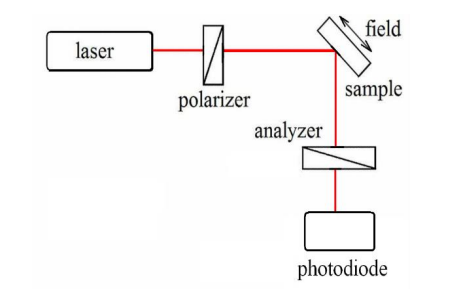
\includegraphics[width=0.6\textwidth]{fig/fig1.png}
    \caption{旋光的解释}\label{fig1}
\end{figure}
唯像的来看,线偏振光可以看成左旋和右旋偏振光的叠加。磁性介质中左旋、
右旋偏振光驱动介质当中电子作左旋和右旋圆周运动,由于磁场的存在,Lorenz
力对电子作用不同导致左旋、右旋光在传播时介质的响应,也就是介电常数不同 ,
因而给出磁光效应。假设一个线偏振的P光(偏振方向平行于入射面)从样品的
表面反射回来,如果样品是完全非磁的,反射回来的光依然是纯粹的P光;如果
样品带有铁磁性,反射光的偏振面相对于入射光的偏振面额外再转过了一个小的
角度,这个小角度称为克尔旋转角$\varPhi '$,因此反射光当中必然会掺杂进去S光的成
分。同时,由于介质对这两种模式的吸收率也不同,从而改变出射光的椭偏率$\varPhi ''$。
由于克尔旋转角$\varPhi '$和克尔椭偏率$\varPhi ''$都是磁化强度$M$的函
数。通过探测克尔旋转角或椭偏率的变化可以推测出磁化强度$M$的变化。 \\
为了获取克尔旋转角$\varPhi '$和克尔椭偏率$\varPhi ''$,我们将两个偏振片在消光角度上
偏离一个小角度$\delta$。这样,光电探头所测到的光强为
\begin{equation}
    I=\left\lvert E_p \sin \delta +E_s\cos \delta \right\rvert ^2 \approx \left\lvert E_p \delta +E_s \right\rvert ^2 
\end{equation}
而 $E_s /E_P = \varPhi ' +i \varPhi ''$,给出Kerr 转角$\varPhi '$和克尔椭偏率$\varPhi ''$,于是有
\begin{equation}
    I = \left\lvert E_p \right\rvert ^2\left\lvert \delta + \varPhi ' +i \varPhi '' \right\rvert ^2 
    \approx  \left\lvert E_p \right\rvert ^2 (\delta ^2 + 2\delta \varPhi ')=I_0(1+\frac{2\varPhi '}{\delta})
\end{equation}
在这里, $I_0=\left\lvert E_p \right\rvert ^2 \delta ^2$, 表示克尔旋转角为零的时候的光强,由于 $\varPhi '$
和 $\varPhi ''$都随着和磁化强度的变化呈线性的变化,所测到的光强随H的变化而变化,表现为
一个磁滞回线的形式。可以通过翻转大于或等于饱和场的磁场得到Kerr 光强的
变化,从而可以得到Kerr转角的饱和值: $\varPhi_m ' = \frac{\delta}{4} \frac{\Delta I}{I_0}$ . \\
磁性薄膜中的磁化强度往往沿着特殊的方向(易磁化轴)自发磁化,如垂直
于膜面或平行于膜面。因此,在实验中通常采取三种简单的构型来测量Kerr信号,
即所谓的纵向克尔效应,横向克尔效应和极向克尔效应。这三种构型是按照光路
与磁化强度相对位置来区分的。$\overrightarrow{M}$位于膜面内,但是垂直于光路的,是横向Kerr效应
(transversal SMOKE), $\overrightarrow{M}$ 垂直于膜面的是极向Kerr效应(polar SMOKE)。极向
Kerr效应最强,纵向Kerr效应要弱很多,横向Kerr效应在一阶近似下没有Kerr转
角和椭偏率,但是以P光(偏振方向平行于入射面)入射的反射光的光强会发生
改变。
\begin{figure}[!h]
    \centering
    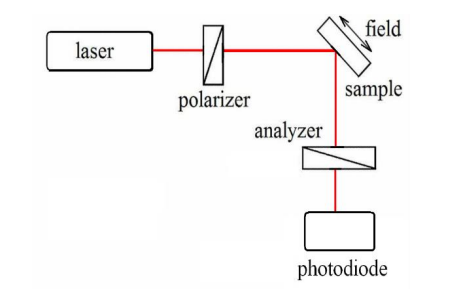
\includegraphics[width=0.6\textwidth]{fig/fig1.png}
    \caption{磁光克尔效应的三种构型}\label{fig2}
\end{figure}
\section{实验内容}
实际实验装置由以下几部分组成:振动隔绝系统(光学平台);磁场(可调电流
源、电磁铁);光路(激光器、起偏器、检偏器、光学调节原件;光电探测器、
光电放大器、万用表);样品座。利用电脑直接控制电磁铁的励磁电流,并同步
读取万用表测量得到的光电压。

\begin{enumerate}
    \item 根据实验需求搭建相对应的光路。
    \item 将二极管激光器控制器安全锁打开,打开电源,将激光强度控制(LD ON)
    和温度控制(TEC ON)都按下,进入工作工作状态。通过调节Optical Power 
    Setpoint来实现激光强度的调节(配合使用设备上Modify键和右侧黑色旋
    钮)。注意,切勿直视激光。
    \item 将光电探测器电源打开(power调至1位置)
    \item 打开光电放大器电源,将显示档调节只光电流选项($I_{PD}$),将量程调制
    mA(Range)。
    \item 打开万用电表。
    \item 打开磁铁电流源(背后红色按钮),并长按前面板Power键,使其进入工
    作状态。
    \item 放置样品,调节样品位置、角度至合适,使得激光光斑能够进入光电探
    测器。注意调节光电放大器量程。
    \item 转动rotary support,调节检偏器偏振方向,使到消光位置,记下极小值
    $I_min$ 。继续旋转,使检偏器离开消光位置数圈,并记下旋转的角度
    (根据实际情况可以适当改变旋转的角度)。rotary support在刻度位于
    标尺中间时,旋转每圈实际走的角度是1.193°。注意调节光电放大器量
    程 (一般在μA档信噪比较好)。  
    \item 打开控制软件,设置磁铁的电流扫描范围,步长等信息,运行测试并保
    存数据。
    \item 测试完成后,关闭激光强度控制(LD)和温度控制(TEC),关闭激光器控
    制器电源;关闭光电探测器,光电放大器,万用表,电磁铁电源,电
    脑。    
\end{enumerate}
\section{实验数据}

\section{误差分析}


\section{思考题}
\subsection*{如何获得椭偏率随磁场变化的曲线?}


\nocite{jiaocai}
\bibliography{ref}
\end{document}